\documentclass[a4paper,10pt]{article}
\usepackage[utf8]{inputenc}
\usepackage{listings}
\usepackage{graphicx}

\title{Rechnernetze Aufgabe 2 Auswertung}

\author{
  Triebe, Marian\\
  \texttt{marian.triebe@haw-hamburg.de}
  \and
  Kirstein, Katja\\
  \texttt{katja.kirstein@haw-hamburg.de}
}

\begin{document}

\maketitle
\tableofcontents
\newpage

\section{Einleitung}
In diesem Dokument wollen wir kurz die Messwerte aus dem
zweiten Rechnernetze Praktikum auswerten und grob analysieren. Außerdem sollen
einige Fragestellungen zu dein einzelnen Testaufbauen beantwortet werden.


%% Setup 1
\section{Setup 1 - Direkte Verbindung zweier Rechner über eine Switch}

\subsection{Aufbau}
Die Kommunikation beider Rechner findet direkt über eine Switch statt. Im Labor war dazu keine weitere Konfiguration nötig, es musste
lediglich das Program \textit{netserver} auf der korrekten Gegenstelle gestartet werden.

\subsection{Ping Messwerte}
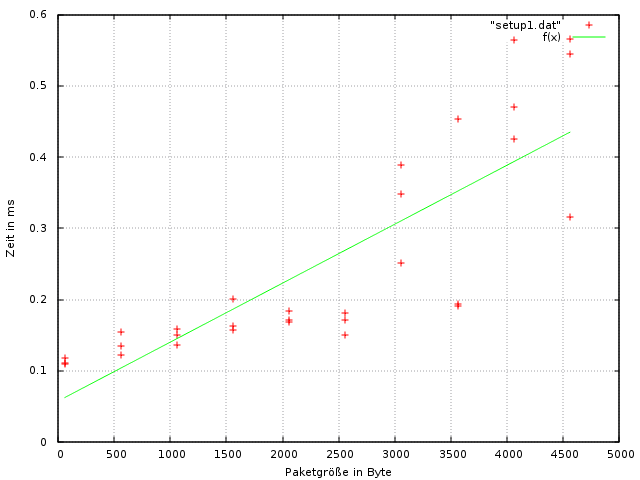
\includegraphics[scale=0.75]{ping_setup1.png}

\subsection{TCP-Übertragung}
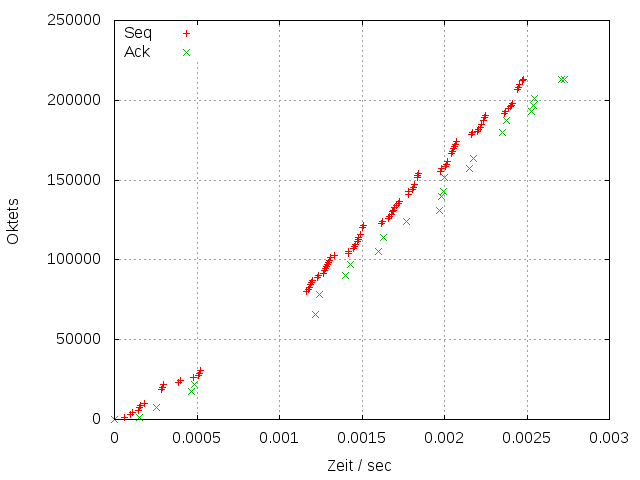
\includegraphics[scale=0.75]{setup1.png}
Die verwendete Paketgröße 65536 Byte.

\subsection{Spezifische Fragen}
\subsubsection{Fragen}
\begin{enumerate}
 \item Wie hoch ist die RTTI in Abhängigkeit von der Paketgröße? Stimmt das mit den Erwartungen überein?
 \item Wie hoch ist die maximale Transferrate bei der Übertragung größerer Datenmengen mit TCP? Entspricht das den Erwartungen? Kann man die Auswirkungen der Algorithmen zur Stauvermeidung erkennen?
 \item Kann man Aussagen treffen zur Arbeitsweise der Switch?
 \item Hat die TCP-Fenstergröße einen Einfluss?
\end{enumerate}
\subsubsection{Antworten}
\begin{enumerate}
 \item Wie auf Abbildung 1 zu erkennen hängt die RTTI (Roundtrip-Time) stark von der Paketgröße ab.
 \item Auf Abbildung 2 ist zu erkennen, dass die Datenrate anfangs niedrig ist und solange keine
 Paketverluste auftraten weiter gesteigert wird. Das deutet auf das \textit{Slow Start} verfahren hin,
 bei diesem Verfahren wird die Übertragungsrate gesteigert bis es zu Paketverlusten kommt. Kommt es zu einem
 Paketverlust, dann wird wieder mit niedriger Datenrate gesendet und sich erneut herangetastet. Das erklärt
 die immer wieder kleinen Steigungen in Abbildung 2.
 \item Wir würden behaupten dass der Switch nach dem \textit{Cut-Through} verfahren arbeitet. Das heißt 
 Pakete die am Switch ankommen werden sofort zum Empfänger weitergeleitet. Fehlerhafte Pakete können somit
 aber erst beim Empfänger erkannt werden.
 \item Ja die TCP-Fenstergröße hat einen Einfluss. Gehen einzelne Pakete mit großer Fenstergröße verloren,
 muss das komplette Paket erneut gesendet werden.
\end{enumerate}


%% Setup 2
\section{Setup 2 - Verbindung über einen Router}

\subsection{Aufbau}
Bei diesem Aufbau war es notwendig mit Hilfe des Befehls \textit{route} eine Route zur Gegenstelle
über einen Router zu machen.

\subsection{Ping Messwerte}
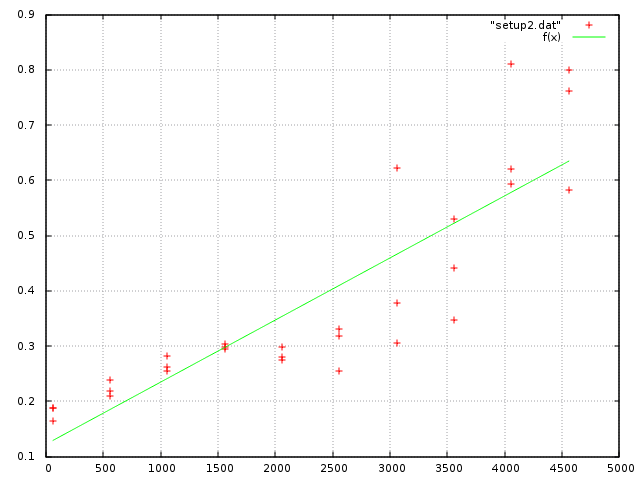
\includegraphics[scale=0.75]{ping_setup2.png}

\subsection{TCP-Übertragung}
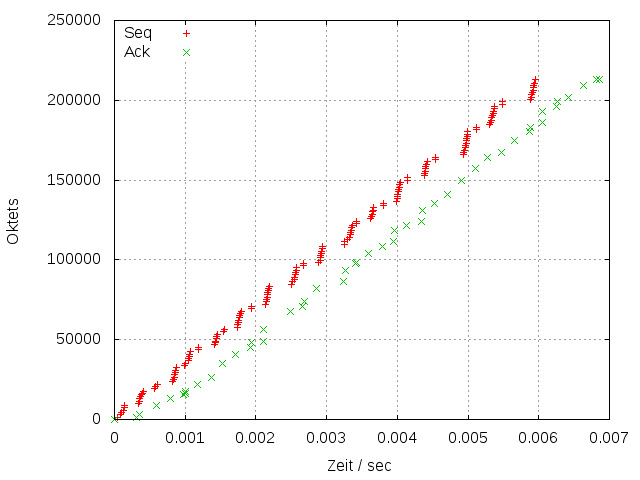
\includegraphics[scale=0.75]{setup2.png}
Die verwendete Paketgröße 65536 Byte.

\subsection{Spezifische Fragen}
\subsubsection{Fragen}
\begin{itemize}
 \item Welchen Einfluss at die Routerperformance auf die RTTI?
 \item Wie verändert sich der Durchsatz?
 \item Welche Eigenschaften haben die Schnittstellen zum Router?
\end{itemize}
\subsubsection{Antworten}
\begin{itemize}
 \item In Abbildung 3 sind keine großen Abweichungen zur vorherigen Messung sichtbar. Das deutet darauf hin
 das der verwendete Router keinen direkten Einfluss auf die Messwerte hatte. Die Routerperformance hatte bei dem
 Ping Test also keine nennenswerten Einflüsse, jedoch kann davon ausgegangen werden, dass schlechte Routerperformance
 sich durchaus auf die Datenrate und den Durchsatz auswirken können.
 \item Der Durchsatz hat sich deutlich verschlechtert. Die \textit{MTU} (Maximum Transmission Unit) bzw. \textit{MMS}
 (Maximum Segment Size) hat sich jedoch nicht verändert und lag wie im Aufbau davor bei 1460 Byte. Bei einer Paketgröße
 von 2058 Bytes hat sich der Durchsatz bei Setup 1 von 390095 Bytes/s auf 234057 Bytes/s verschlechtert.
 \item Die Schnittstellen zum Router haben eine Übertragungsrate von 1GBit/s.
\end{itemize}


%% WAN1
\section{WAN-Verbindung 1}

\subsection{Aufbau}
Die erste WAN Konfiguration soll über den Gateway \textit{192.168.17.240} bzw. \textit{192.168.18.240} gehen. Dazu werden
an der Gegenstelle sowie am Sendenden PC die Pfade per \textit{route} Befehl konfiguriert.

\subsection{Ping Messwerte}
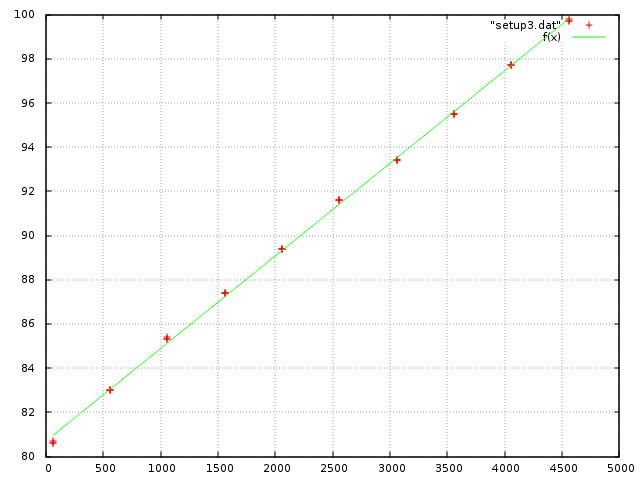
\includegraphics[scale=0.75]{ping_setup_wan1.png}

\subsection{TCP-Übertragung}
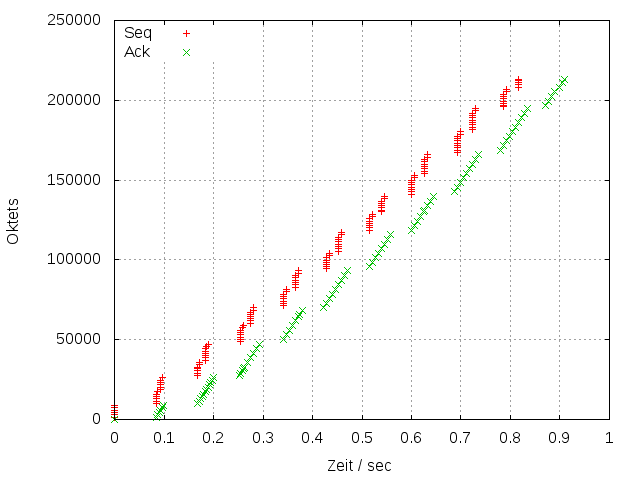
\includegraphics[scale=0.75]{setup_wan1.png}
Die verwendete Paketgröße 65536 Byte.

\subsection{Windowsize}
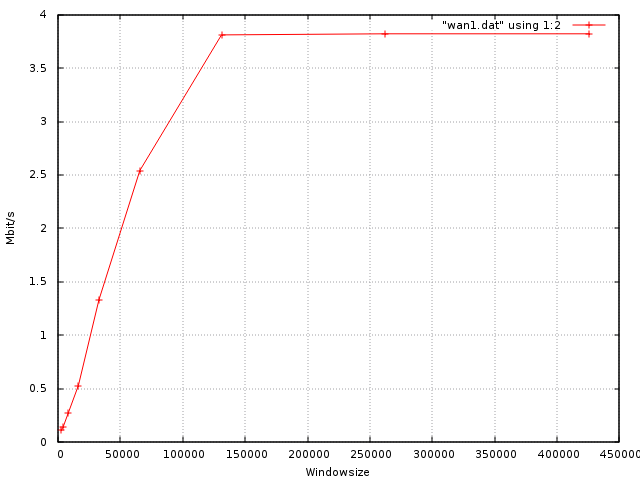
\includegraphics[scale=0.75]{wan1_windows.png}

\subsection{Spezifische Fragen}
\begin{itemize}
 \item Wie in der Abbildung von 4.2 zu erkennen, liegt die RTTI zwischen 80 und 100 Millisekunden.
 \item {Zum Berechnen der Strecke nehmen wir folgende Formel
 \begin{equation}
  l=RTTI*2/3*c
 \end{equation}
 Setzt man für die RTTI nun 80 Millisekunden ein und für c die Lichtgeschwindigkeit in Meter/s,
 so erhällt man eine Strecke der Länge von 15989 Kilometern.}
 \item Die erwartete Windowsize zum ausnutzen der Leitung liegt bei ca. 13271 Bytes.
 \item Wie in 4.4 zu sehen ist, wird die Bandbreite erst ab einer Fenstergröße von etwas mehr als 130000 byte vollständig ausgenutzt.
 \item Die maximale Übertragungsgeschwindigkeit lag bei 3.82 Mbit/s
\end{itemize}

%% WAN2
\section{WAN-Verbindung 2}

\subsection{Aufbau}
Die zweitee WAN Verbindung wird mit dem Gateway \textit{192.168.17.241} bzw. \textit{192.168.18.241} auf den PCs wie bei WAN 1 mit dem route Befehl eingerichtet.

\subsection{Ping Messwerte}
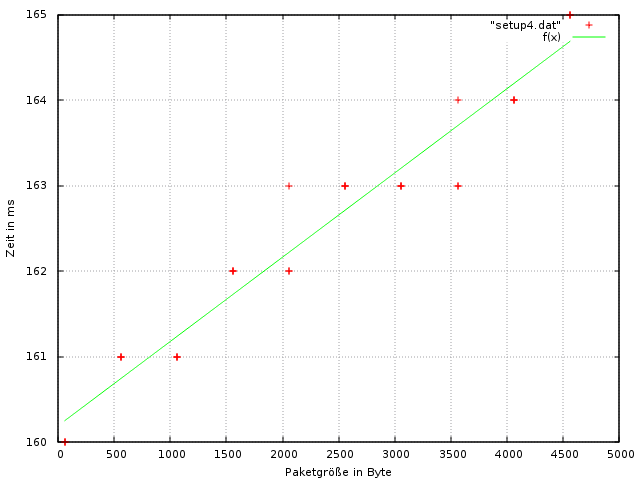
\includegraphics[scale=0.75]{ping_setup_wan2.png}

\subsection{TCP-Übertragung}
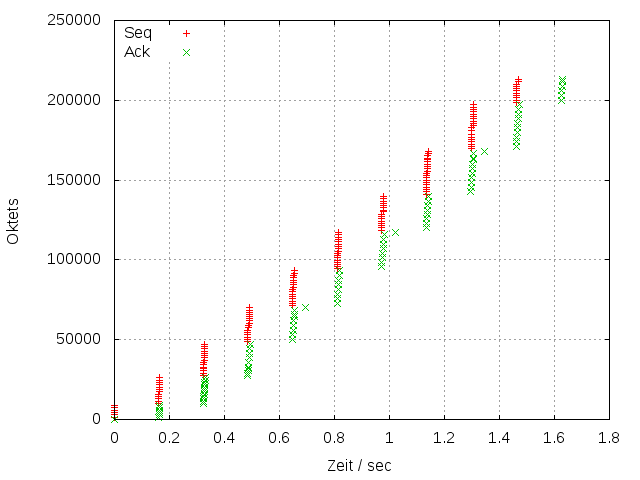
\includegraphics[scale=0.75]{setup_wan2.png}
Die verwendete Paketgröße 65536 Byte.

\subsection{Windowsize}
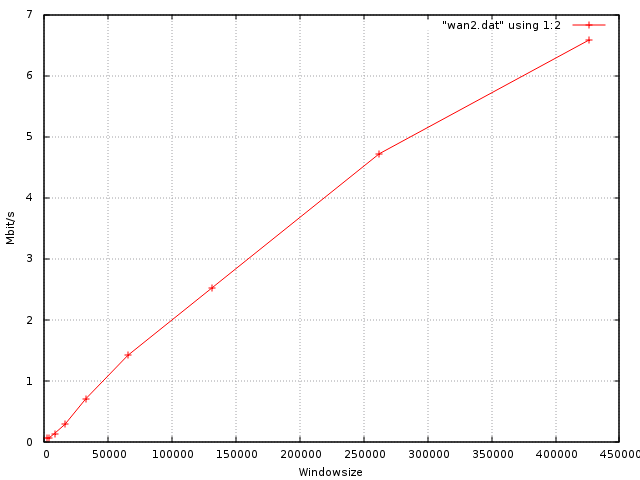
\includegraphics[scale=0.75]{wan2_windows.png}

\subsection{Spezifische Fragen}
\begin{itemize}
 \item Aus der Abbildung von 5.2 ist zu erkennen, dass die RTTI zwischen 160 und 165 Millisekunden liegt.
 \item {Formel zum Berechnen der Strecke: 
 \begin{equation}
  l=RTTI*2/3*c
 \end{equation}
 Mit dem RTTI von 160 ergibt sich eine Strecke von 31998 Kilometern.
 \item In der Abblidung aus 5.4 kann man eine maximale Fenstergröße von 425984 Byte. Das Diagramm hört leider dort auf, 
 für weitere Vergewisserung müsste eine erneute Messung durchegführt werden.}
 \item Die maximale Übertragungsgeschwindigkeit lag bei 6.58 Mbit/s
\end{itemize}

%% WAN3
\section{WAN-Verbindung 3}

\subsection{Aufbau}
Die dritte WAN-Verbindung wird wie die Zwei vorherigen eingestellt, diesesmal mit dem Gateway \textit{192.168.17/18.242}

\subsection{Ping Messwerte}
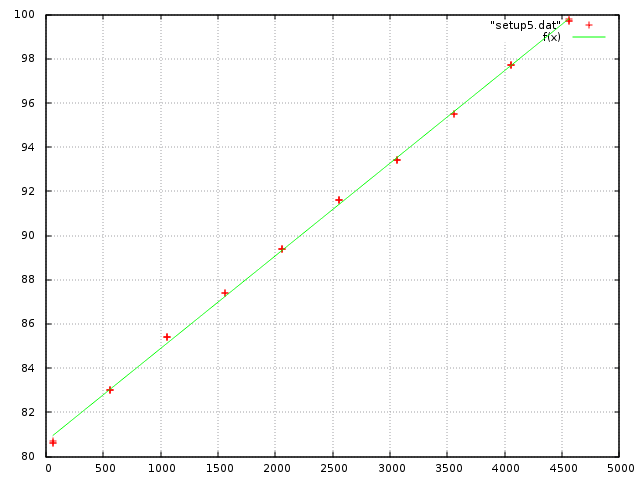
\includegraphics[scale=0.75]{ping_setup_wan3.png}

\subsection{TCP-Übertragung}
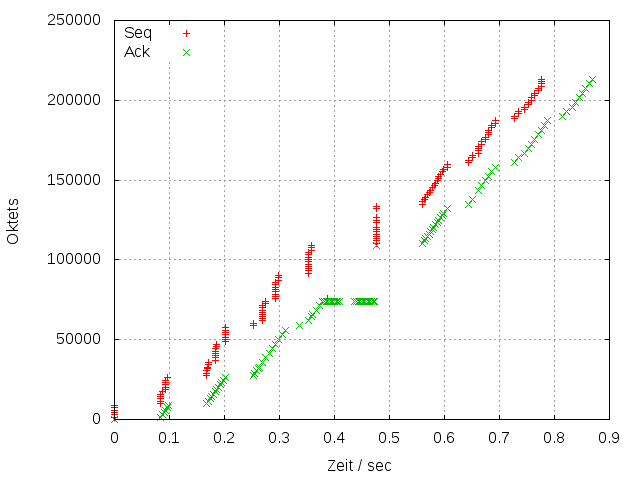
\includegraphics[scale=0.75]{setup_wan3.png}
Die verwendete Paketgröße 65536 Byte.
Wie zu sehen wird das 150 Paket verworfen und erneut versendet.

\subsection{Windowsize}
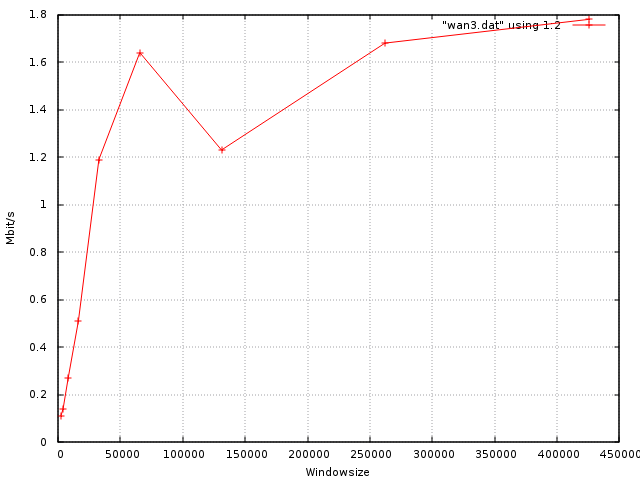
\includegraphics[scale=0.75]{wan3_windows.png}

\subsection{Spezifische Fragen}
\begin{itemize}
 \item Aus der Abbildung von 6.2 ist zu erkennen, dass die RTTI zwischen 80 und 100 Millisekunden liegt.
 \item Formel zum Berechnen der Strecke: 
 \begin{equation}
  l=RTTI*2/3*c
 \end{equation}
 Mit der Formel kommt man auf eine Strecke von 15989 Kilometern.
 \item Die Abblidung aus  6.4 zeigt wie die Fenstergröße von 65536 erreicht wird, und das darauf folgende Paket
 weggeworfen wird, bei dieser fehlerhaften Verbindung.
 \item Die maximale Übertragungsgeschwindigkeit lag bei 1.78 Mbit/s
\end{itemize}

%% WAN4
\section{WAN-Verbindung 4}

\subsection{Aufbau}
Mit dem Gateway \textit{192.168.17.243} und \textit{192.168.18.243} wird diese wie alle anderen konfiguriert

\subsection{Ping Messwerte}
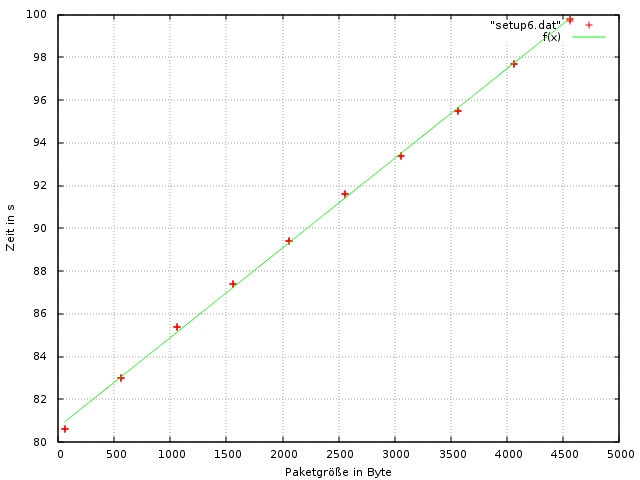
\includegraphics[scale=0.75]{ping_setup_wan4.png}

\subsection{TCP-Übertragung}
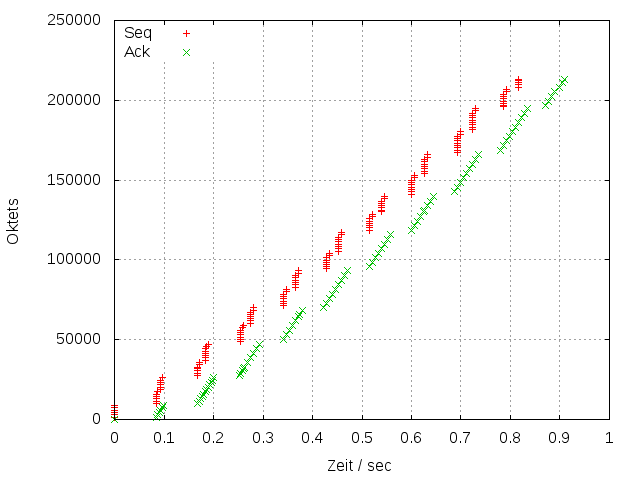
\includegraphics[scale=0.75]{setup_wan4.png}
Die verwendete Paketgröße 65536 Byte.

\subsection{Windowsize}
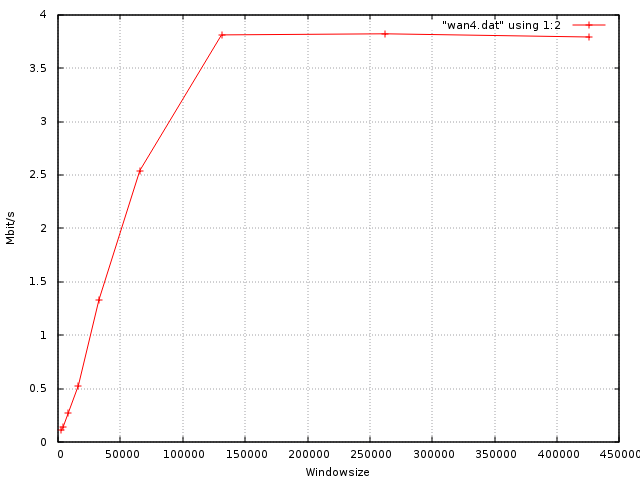
\includegraphics[scale=0.75]{wan4_windows.png}

\subsection{Spezifische Fragen}
\begin{itemize} 
 \item Aus der Abbildung von 5.2 ergibt sich eine RTTI zwischen 80 und 100 Millisekunden.
 \item {Formel zum Berechnen der Strecke: 
 \begin{equation}
  l=RTTI*2/3*c
 \end{equation}
 Man kommt wieder auf die selbe Entfernung von 15989 Kilometern.
 \item Wie in der Abblidung 7.4 zu sehen, ist die ideale Fenstergröße 131072 Byte um die Verbindung auszunutzen.}
 \item Die maximale Übertragungsgeschwindigkeit lag bei 3.82 Mbit/s
\end{itemize}
 
\end{document}
